\documentclass[letterpaper]{article}
%\usepackage[pass,showframe]{geometry}

\usepackage{ijcai17}
\usepackage{times}
\usepackage{graphicx}
\usepackage{cleveref}

\usepackage{subfigure}

\usepackage[ruled,vlined]{algorithm2e}
\usepackage{MnSymbol,wasysym}
\usepackage{latexsym}
\usepackage{algpseudocode}
\usepackage{amsmath}

\usepackage{tikz}

\usetikzlibrary{graphs}

\newcommand{\citet}[1]{\citeauthor{#1} \shortcite{#1}}
\newcommand{\citep}[1]{\cite{#1}}

\newcommand{\AlgVar}[1]{\mathit{#1}}

\newcommand{\McSplit}{\textproc{McSplit}}

\newcommand{\nmax}{n_{\max}}

\newcommand{\lineref}[1]{line~\ref{#1}}
\newcommand{\linerangeref}[2]{lines~\ref{#1} to~\ref{#2}}
\newcommand{\Lineref}[1]{Line~\ref{#1}}
\newcommand{\Linerangeref}[2]{Lines~\ref{#1} to~\ref{#2}}

% TODO: use operatorname for these
\DeclareMathOperator{\V}{V}
\DeclareMathOperator{\E}{E}
\DeclareMathOperator{\N}{N}
\DeclareMathOperator{\vtxlabel}{label}

\newcommand{\BigO}[1]{\ensuremath{\operatorname{O}\left(#1\right)}}

%\newcommand{\examplexG}[5] {
%    \begin{minipage}{.2\textwidth}
%    \tikz {
%        \graph [nodes={draw, circle, minimum width=.6cm}, circular placement, radius=1cm,
%                clockwise=5] {
%                    1[label=90:#1],2[label=0:#2],3[label=0:#3],4[label=180:#4],5[label=180:#5];
%            1--4; 1--5; 2--3; 2--5; 3--5;
%        };
%    }
%    \end{minipage}
%}
%\newcommand{\examplexH}[6] {
%    \begin{minipage}{.2\textwidth}
%    \tikz {
%        \graph [nodes={draw, circle, minimum width=.6cm}, circular placement, radius=1.1cm,
%                clockwise=6, phase=60] {
%                    a[label=0:#1],b[label=0:#2],c[label=0:#3],d[label=180:#4],e[label=180:#5],f[label=180:#6];
%            a--b; a--c; a--e; b--d; b--f; c--d; c--e; c--f; d--f; e--f;
%        };
%    }
%    \end{minipage}
%}

\title{A Partitioning Algorithm for Maximum Common Subgraph Problems\thanks{This work
was supported by a pile of money from a funding agency.}}
\author{The Anonymous Authors of Paper 2431 \\
Academy of Anonymous Academics, Some City, Some Country \\
anonymous@anonymous.anonymous}

\begin{document}

\maketitle

\begin{abstract}
    We introduce a new branch and bound algorithm for the maximum common
    subgraph and maximum common connected subgraph problems which is based
    around vertex labelling and partitioning. Our method in some ways resembles
    a traditional constraint programming approach, but uses a novel compact
    domain store and supporting inference algorithms which dramatically reduce
    the memory and computation requirements during search, and allow better
    dual viewpoint ordering heuristics to be calculated cheaply.  Experiments
    show a speedup of more than an order of magnitude over the state of the
    art, and demonstrate that we can operate on much larger graphs without
    running out of memory.
\end{abstract}

\section{Introduction}

To determine the similarity or difference between two graphs, we must first
find what they have in common
\citep{DBLP:journals/prl/Bunke97,DBLP:journals/prl/FernandezV01,KriegeThesis}.
The \emph{maximum common subgraph} family of problems involves finding a large
graph which is isomorphic to subgraphs of two given graphs simultaneously.
Because graphs are widely used to model real-world phenomena, maximum common
subgraph problems have arisen in molecular science (where graphs represent
molecules)
\citep{DBLP:journals/jcamd/RaymondW02a,Ehrlich:2011,DAM2014,Grindley1993707},
computer vision \cite{DBLP:journals/jair/CookH94}, discovery of repeated
patterns in source code \cite{DBLP:journals/tkde/DjokoCH97} and circuits
\cite{DBLP:journals/jair/CookH94}, and recognition of handwritten characters
\cite{SIWEILU1991617}.

Maximum common subgraph problems are NP-hard, and remain challenging
computationally. Recent practical progress has been made by using constraint
programming \citep{DBLP:conf/cp/NdiayeS11,DBLP:conf/cp/McCreeshNPS16}, by
reducing to the maximum clique problem
\citep{LeviG,DBLP:conf/cp/McCreeshNPS16}, and by adapting subgraph isomorphism
algorithms \citep{UpcomingAAAIPaper}. This paper introduces a new branch and
bound algorithm which exploits special properties of these problems to allow a
much faster exploration of the search space, whilst retaining the filtering and
bounding benefits of the constraint programming approach. We describe the
algorithm for the basic maximum common subgraph problem, and discuss how it may
be adapted to handle vertex labels, edge labels, and the requirement that the
found subgraph be connected. We then present an empirical study of the
algorithm, demonstrating that it improves the state of the art by more than an
order of magnitude on the unlabelled variant of the problem, and showing that
it can handle much larger instances than earlier constraint programming or
clique approaches due to lower memory usage.

\section{Preliminaries}

We initially assume that graphs are unlabelled, undirected and without loops
(Section~\ref{sec:extensions} describes how these restrictions may be relaxed).
The vertices and edge sets of a graph $G$ are denoted $\V(G)$ and $\E(G)$.  The
set of vertices adjacent to vertex $v$ in graph $G$ is called the
\emph{neighbourhood} of $v$, and denoted $\N(v, G)$.  The graph $\overline{G}$
is the complement of $G$, obtained copying the vertices of $G$ and adding an
edge between each pair of distinct vertices if and only if $G$ does not
have an edge between the corresponding pair.

Let $G$ and $H$ be the two input graphs to our maximum common subgraph problem.
The orders (vertex counts) of these graphs are denoted $n_G$ and $n_H$. We will
use $n$ in complexity results to denote $\max(n_G + n_H)$.

\section{Prior Work}

The most successful existing approaches to solving MCS are reformulation to the
maximum clique problem on one hand \cite{DBLP:conf/cp/McCreeshNPS16}, and
constraint programming on the other \cite{DBLP:conf/cp/NdiayeS11}. In the
clique encoding, an association graph is created with one node for each pair in
the set $\{(u,v) \mid u \in \V(G), v \in \V(H) \}$ and an edge for each pair of
mappings that may be chosen together. A maximum clique in this graph
corresponds directly to a maximum common subgraph of $G$ and $H$.

In the constraint programming approach  \cite{DBLP:conf/cp/NdiayeS11}, a variable corresponds to
each vertex in $G$, and each variable initially has one value in its domain for
each vertex in $H$ to which it may be mapped, plus an additional value $\bot$
signifying that the vertex remains unmapped. A backtracking search is performed
in which values are assigned to variables, and propagation rules are used to
remove infeasible values from domains.
\textit{A matching algorithm propagates
a soft global allDifferent constraint which maximizes the number variables that are assigned to values different from $\bot$, while ensuring they are all different when they are not assigned to $\bot$.
Different constraint propagation techniques are compared in \cite{DBLP:conf/cp/NdiayeS11}. The combination ``MAC+Bound'' (resp. ``FC+Bound'') obtains the best results on labelled (resp. non labelled) graphs and outperforms the approach of \cite{McGreg82} and the CP model of \cite{DBLP:conf/mco/VismaraV08}. The combination ``MAC+Bound'' maintains arc consistency~\cite{sabi94} of edge constraints, whereas the conbination ``FC+Bound'' simply performs forward-checking on these constraints. In both combinations, the ``Bound'' filtering checks whether it is possible to assign distinct values to enough variables to surpass the best cost found so far (it is a weaker version of GAC(\emph{softAllDiff}) \cite{peti01} which computes the maximum number of variables that can be assigned distinct values).}

\section{The \McSplit\ algorithm}

We now present \McSplit, a branch and bound algorithm 
which uses a new vertex-labelling scheme to avoid explicitly maintaining the
set of feasible mappings for each vertex in $\V(G)$. 
\iffalse
As we will explore in
Section~\ref{sec:comparison}, the algorithm may be viewed as a version of the
constraint programming forward-checking (CP-FC) algorithm using a compact data
structure that exploits the nature of the MCS problem.  It is sufficiently
different, however, that it is helpful to describe the algorithm without
reference to previous approaches.

%At each node of the search tree, the algorithm
%labels vertices in $\V(G)$ and $\V(H)$ such that a pair $(v, w)$ with $v \in
%\V(G)$ and $w \in \V(H)$ can be added to the mapping if and only if $v$ and $w$
%have the same label.
\fi
\McSplit\ finds a maximum-cardinality mapping $M^* = \{(v_1, w_1), \dots,
(v_{|M^*|}, w_{|M^*|})\}$, where the $v_i$ are distinct members of $\V(G)$ and the
$w_i$ are distinct vertices of $\V(H)$, such that $v_i$ and $v_j$ are adjacent
in $G$ if and only if $w_i$ and $w_j$ are adjacent in $H$. 
Given such a mapping, the subgraph of $G$ induced by $\{v_i, \dots, v_{|M^*|}\}$
and the subgraph of $H$ induced by $\{w_i, \dots, w_{|M^*|}\}$ are a maximum
common subgraph.

We will use the graphs $G$ and $H$ in Figure~\ref{fig:alg1} to demonstrate the
algorithm.  These graphs have a maximum common subgraph with four vertices; one
example is the mapping $\{1a, 2f, 3d, 5b\}$ where vertex $1$ is assigned to
vertex $a$, $2$ is assigned to $f$, $3$ to $d$ and $5$ to $b$.

\begin{figure}[ht]
\centering
    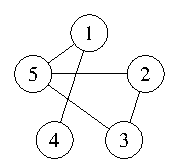
\includegraphics{graph_G}
    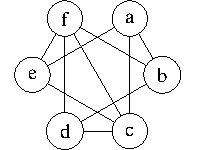
\includegraphics{graph_H}
%    \examplexG{}{}{}{}{}
%    \examplexH{}{}{}{}{}{}
\caption{Graphs $G$ and $H$}
\label{fig:alg1}
\end{figure}

The algorithm builds up a mapping $M$, starting with the empty mapping
$\emptyset$. Select a vertex in $\V(G)$ as the first vertex to be mapped; in
our example we will arbitrarily choose vertex $1$. Each of the vertices in
$\V(H)$ to which vertex $1$ may be mapped will be tried in turn, and finally the
possibility where vertex $1$ remains unmatched will be tried.

We begin by mapping vertex $1$ to vertex $a$, giving $M=\{1a\}$.  Now label
each unmatched vertex according to whether it is adjacent to vertex $1$ (in
$G$) or vertex $a$ (in $H$), as shown in Figure~\ref{fig:alg2}.  Adjacent
vertices have label 1; non-adjacent vertices have label 0.  We can extend $M$
with a vertex mapping $vw$, with $v \in \V(G)$ and $w \in \V(H)$, if and only
if $v$ and $w$ have the same label.  This property, that two vertices may be
mapped together if and only if they share a label, is the algorithm's main
invariant.

\begin{figure}[ht]
\centering
\begin{minipage}[t]{0.15\linewidth}
    Mapping

    \bigskip

    $\{1a\}$
\end{minipage}
\quad
\begin{minipage}[t]{0.3\linewidth}
    Labelling of $G$
    \begin{tabular}[t]{cc}
    \hline
        Vertex & Label\\
    \hline
        $2$ & 0 \\
        $3$ & 0 \\
        $4$ & 1 \\
        $5$ & 1 \\
    \hline
    \end{tabular}
\end{minipage}
\quad
\begin{minipage}[t]{0.3\linewidth}
    Labelling of $H$
    \begin{tabular}[t]{cc}
    \hline
        Vertex & Label\\
    \hline
        $b$ & 1 \\
        $c$ & 1 \\
        $d$ & 0 \\
        $e$ & 1 \\
        $f$ & 0 \\
    \hline
    \end{tabular}
\end{minipage}
    \caption{Labels on vertices after mapping $1$ to $a$}
\label{fig:alg2}
\end{figure}

Next, extend the mapping by pairing a vertex in $G$ with a vertex in $H$ of the
same label; we will choose to map vertex $2$ to vertex $d$, giving $M=\{1a,
2d\}$ (Figure~\ref{fig:alg3}).  Each unmapped vertex $v \in \V(G)$ is labelled
with a two-character bit string, indicating its adjacency to each of
the two mapped vertices in $\V(G)$ (vertices $1$ and $2$).  For example, vertex
$3$ is labelled $01$, indicating that it is not adjacent to vertex $1$ but is adjacent
to vertex $2$.  Labels are given to unmapped vertices in $\V(H)$ in a similar fashion,
showing adjacency to matched vertices $a$ and $d$.

Our invariant is maintained: we can extend $M$ by a vertex pairing if and only
if the two vertices have the same label. Note also that the labels can be
calculated efficiently, since each label (in Figure~\ref{fig:alg3}) is prefixed
by the label at the previous level of the search tree (Figure~\ref{fig:alg2}).

\begin{figure}[ht]
\centering
\begin{minipage}[t]{0.15\linewidth}
    Mapping

    \bigskip

    $\{1a, 2d\}$
\end{minipage}
\quad
\begin{minipage}[t]{0.3\linewidth}
    Labelling of $G$
    \begin{tabular}[t]{cc}
    \hline
        Vertex & Label\\
    \hline
        $3$ & 01 \\
        $4$ & 10 \\
        $5$ & 11 \\
    \hline
    \end{tabular}
\end{minipage}
\quad
\begin{minipage}[t]{0.3\linewidth}
    Labelling of $H$
    \begin{tabular}[t]{cc}
    \hline
        Vertex & Label\\
    \hline
        $b$ & 11 \\
        $c$ & 11 \\
        $e$ & 10 \\
        $f$ & 01 \\
    \hline
    \end{tabular}
\end{minipage}
\caption{After mapping $2$ to $d$}
\label{fig:alg3}
\end{figure}

The algorithm backtracks when the incumbent, i.e. the largest matching found so far, is at least as large
as a calculated bound given $M$ and the current labelling. To demonstrate how
this bound is calculated, we consider the situation one level deeper in the
search tree shown in Figure~\ref{fig:alg4}.

\begin{figure}[ht]
\centering
\begin{minipage}[t]{0.2\linewidth}
    Mapping

    \bigskip

    $\{1a, 2d, 3f\}$
\end{minipage}
\quad
\begin{minipage}[t]{0.3\linewidth}
    Labelling of $G$
    \begin{tabular}[t]{cc}
    \hline
        Vertex & Label\\
    \hline
        $4$ & 100 \\
        $5$ & 111 \\
    \hline
    \end{tabular}
\end{minipage}
\quad
\begin{minipage}[t]{0.3\linewidth}
    Labelling of $H$
    \begin{tabular}[t]{cc}
    \hline
        Vertex & Label\\
    \hline
        $b$ & 111 \\
        $c$ & 111 \\
        $e$ & 101 \\
    \hline
    \end{tabular}
\end{minipage}
\caption{After mapping $3$ to $f$}
\label{fig:alg4}
\end{figure}

Three vertex labels are used: 100,
101, and 111.  The first two of these only appear in one graph, and therefore
there is no way to add a pair of vertices with label 100 or 101 to the mapping.
The final label, 111, appears once in $G$ and twice in $H$, and therefore at
most one pair with this label can be added to $M$.  Thus, the upper bound on
matching size is $|M| + 1 = 4$. The general formula for the upper bound is
as follows, where $L$ is the set of labels used in both graphs.

\begin{multline*}
    \mathit{bound} = |M| + \sum_{l \in L} \min\big(|\{ v \in \V(G) : \vtxlabel(v)=l\}|, \\
        |\{ v \in \V(H) : \vtxlabel(v)=l \}|\big)
\end{multline*}


%When we have explored the full
%search space of matchings containing $\{1a, 2d\}$, we try reassigning $2$ to
%$f$.  Since $d$ and $f$ are the only vertices to which $2$ can be matched given
%the decision to match $1$ to $a$, we lastly explore the possibility that $2$ is
%left unmatched, by giving $2$ the label $\bot$ and selecting another vertex in
%$\V(G)$ to assign.

\paragraph{Efficient representation of label classes} The algorithm as
described so far requires $\BigO{n^2}$ space at each level of the search tree,
since labels may be up to $n_G$ bits in length. We can reduce the memory
requirement to $\BigO{n}$ per level by storing a \emph{label class} as a pair
$\langle P,T \rangle$ for each label $l$ that is used, where $P$ is the set of
vertices in $\V(G)$ labelled $l$, and $T$ is the set of vertices in $\V(H)$
labelled $l$.\footnote{We adopt terminology from subgraph isomorphism where one
graph is a pattern graph $P$ and the other the target graph $T$.} Since there
are $n_G + n_H$ vertices in the two graphs, at most $n_G + n_H$ label classes
can exist at once, and there are at most $n_G + n_H$ vertices in the union of
all of the $P$ and $T$ sets.  We can gain further efficiency by discarding
during search any label class that has an empty $P$ or $T$ set.

\begin{algorithm}[ht]
\DontPrintSemicolon
\nl $\FuncSty{expand}(\AlgVar{future},M)$ \;
\nl \Begin{
%\nl \lIf {$\AlgVar{future} = \emptyset$ \bf{and} $|M| > |\AlgVar{incumbent}|$}
\nl \lIf {$|M| > |\AlgVar{incumbent}|$}{$save(matching)$} \label{StoreIncumbent}
%\nl \lIf {$\AlgVar{future} = \emptyset$}{return}
\nl $bf \gets 0$ \label{SetBestFutureToZero} \;
\nl \lFor {$\langle P,T \rangle \in \AlgVar{future}$}{$\AlgVar{bf} \gets \AlgVar{bf} + \min(|P|,|T|)$}
\nl \lIf {$|M|  + \AlgVar{bf} \leq |\AlgVar{incumbent}|$}{return} \label{PruneSearch}
\bigskip
\nl $\langle P,T \rangle \gets \FuncSty{SelectLabelClass}(\AlgVar{future})$ \label{SelectClass} \;
\nl $v \gets \FuncSty{SelectVertex}(P)$ \label{SelectVertex} \;
\nl \For {$w \in T$ \label{WLoop}} {
\nl    $M \gets M \cup (v,w)$ \label{GrowM} \;
\nl    \bf{Let} $\AlgVar{future'} \gets \emptyset$ \label{NewFuture} \;
\nl    \For {$\langle P',T'\rangle \in future$ \label{InnerLoop}}{
\nl        \bf{Let} $P'' \gets P' \cap N(v,G) \setminus \{v\}$ \label{NewPWithEdge} \;
\nl        \bf{Let} $T'' \gets T' \cap N(w,H) \setminus \{w\}$ \;
\nl        \If {$P'' \neq \emptyset$ \bf{and} $T'' \neq \emptyset$}
        {$\AlgVar{future'} \gets \AlgVar{future'} + \langle P'' , T'' \rangle$ \label{AddToFutureWithEdge}}
\nl        \bf{Let} $P'' \gets P' \cap N(v,\overline{G}) \setminus \{v\}$ \label{NewPWithoutEdge}  \;
\nl        \bf{Let} $T'' \gets T' \cap N(w,\overline{H}) \setminus \{w\}$ \;
\nl        \If {$P'' \neq \emptyset$ \bf{and} $T'' \neq \emptyset$}
        {$\AlgVar{future'} \gets \AlgVar{future'} + \langle P'' , T'' \rangle$} \label{InnerLoopEnd}
       }
\nl   $\FuncSty{expand}(\AlgVar{future'},M)$ \label{ExpandWithV} \;
\nl   $M \gets M \setminus \{(v,w)\}$ \label{ShrinkM} \;
  }
\nl $P' \gets P \setminus \{v\}$ \label{RemoveV} \;
\nl $\AlgVar{future} \gets \AlgVar{future} \setminus \{\langle P,T \rangle\}$\;
\nl \lIf {$P' \neq \emptyset$} {$\AlgVar{future} \gets \AlgVar{future} \cup \{\langle P',T \rangle \}$}
\nl $\FuncSty{expand}(\AlgVar{future},M)$ \label{ExpandWithoutV} \;
}
\;
\nl $\FuncSty{McSplit}(G,H)$ \label{McSplitFun} \;
\nl \Begin{
\nl $\AlgVar{incumbent} \gets \emptyset$ \;
\nl $\FuncSty{expand}(\{\langle V(G),V(H) \rangle \},\emptyset)$ \label{FirstExpandCall} \;
\nl return $|\AlgVar{incubent}|$ \;
}
\caption{\McSplit\ algorithm for Maximum Common Subgraph}
\label{McCliqueAlg}
\end{algorithm}

\paragraph{Algorithm \ref{McCliqueAlg} Explained} The recursive procedure, $\FuncSty{expand}$, has
two parameters.  The parameter $\AlgVar{future}$ is a list of label classes,
each represented as a $\langle P, T \rangle$ pair as described above.  The
parameter $M$ is the current mapping of vertices.  On each call to
$\FuncSty{expand}$, the invariant holds that a $(v,w)$ pair may be added to $M$
if and only if $v$ and $w$ belong to the same label class in $M$.

\Lineref{StoreIncumbent} stores the current mapping $M$ if it is large enough
to unseat the incumbent.  \Linerangeref{SetBestFutureToZero}{PruneSearch} prune
the search when a calculated upper bound (best future $\AlgVar{bf}$ plus $|M|$) is not larger
than the incumbent.

The remainder of $\FuncSty{expand}$ performs the search.  A label class
$\langle P, T \rangle$ is selected from $\AlgVar{future}$, where $P \subseteq V(G)$ and $T \subseteq V(H)$,
using some heuristic (\lineref{SelectClass}).  From this label class, a
vertex $v$ is selected from $P$ using a heuristic (\lineref{SelectVertex}). We now
iterate over all possible vertices in $T$ (\linerangeref{WLoop}{ShrinkM}). A
vertex $w \in T$ is selected and mapping $M$ is extended (\lineref{GrowM}). A
new set of label-classes, $\AlgVar{future'}$, is created (\lineref{NewFuture}).
Every label-class in $\AlgVar{future}$ can now be split
(\linerangeref{InnerLoop}{InnerLoopEnd}) into two new classes. The first of
these classes (\linerangeref{NewPWithEdge}{AddToFutureWithEdge}) contains
vertices in $P$ adjacent to $v$ and vertices in $T$ adjacent to $w$.  This is
added to $\AlgVar{future'}$ if both sets contain at least one vertex.  This is
then repeated symmetrically for non-adjacency
(\linerangeref{NewPWithoutEdge}{InnerLoopEnd}) using the compliments of the
graphs.  A recursive call is then made (\lineref{ExpandWithV}), on return from
which we remove the mapping $(v,w)$.  Having explored all possible mappings of
$v$ with vertices in $T$ we now consider what happens if $v$ is not matched
(\linerangeref{RemoveV}{ExpandWithoutV}). Note that removing $v$ from its label
class is equivalent to matching vertex $v$ to the null vertex $\bot$.

We start our search at the function $\FuncSty{McSplit}$ (\lineref{McSplitFun}),
with graphs $G$ and $H$ as inputs.  This function returns the size of the
largest mapping.  In \lineref{FirstExpandCall} the initial call is made to
$\FuncSty{expand}$; at this point we have a single label-class containing all
vertices, and the mapping $M$ is empty.

\iffalse
\paragraph{Heuristics} We ran a small experiment comparing lots of heuristics
such as \dots on random instances. The one where you choose a label class with
as small a max(left size, right size) as possible seemed to work best. ? Why?
\fi

\section{Comparison with Existing Algorithms}\label{sec:comparison} The
\McSplit\ algorithm may be considered as a version of the constraint
programming, forward-checking (CP-FC) algorithm of
\citep{DBLP:conf/cp/NdiayeS11}, using an efficient, compressed representation
of domains.  (Recall that in the CP-FC algorithm, each vertex in $v \in \V(G)$
is represented by a variable, whose domain corresponds to the set of vertices
in $\V(H)$ to which $v$ may currently be mapped.)

Given a label class $\langle P,T \rangle$ in \McSplit\, the vertices in $P$
correspond to variables in CP-FC, all of which have domain equal to $T$.  The
label-class representation of domains is possible because throughout the CP-FC
algorithm for max common subgraph, the domains of any two variables are either
identical or disjoint.  (To the best of our knowledge, this observation has
not been made previously.)

Where CP-FC uses a soft allDifferent constraint to filter and compute a bound,
\McSplit\ computes a bound from each label class in the future, i.e. it
performs Hall Set reasoning on the fly.

\McSplit\ requires $\BigO{n}$ time at each search node, and does not require
any auxiliary data structures larger than the adjacency matrices of $G$ and $H$
to be built prior to search.  CP-FC requires $\BigO(?????)$ \dots The clique
encoding requires an association graph with $n_G n_H$ vertices to be
constructed before search.  Modern maximum-clique algorithms typically perform
a colouring step at each search node that is quadratic in the order of the
graph, and thus $\BigO{n^4}$ in the order of the max common subgraph input
graphs.

? Mention partition backtracking

The correctness of \McSplit\ can be seen by noting its equivalence to CP-FC
\citep{DBLP:conf/cp/NdiayeS11}, if we replace the label-class representation of
$\mathit{future}$ with domain stores in Algorithm \ref{McCliqueAlg}.  To obtain
the CP-FC algorithm, replace \linerangeref{InnerLoop}{InnerLoopEnd} of
Algorithm \ref{McCliqueAlg} with Algorithm \ref{cpAlg}.  The pruning of domains
carried out in these lines can be easily seen to be equivalent to the
corresponding lines in Algorithm \ref{McCliqueAlg}.

\begin{algorithm}
\DontPrintSemicolon
\nl    \For {$u \in \N(b,G)$}{
\nl        remove $v$ from $D'_u$ \;
\nl        remove the inverse neighbourhood of $t$ from $D'_u$ \;
       }
\nl    \For {$u \in \N(b,\overline{G})$}{
\nl        remove $v$ from $D'_u$ \;
\nl        remove the neighbourhood of $t$ from $D'_u$ \;
       }
\caption{Replacement for \linerangeref{InnerLoop}{InnerLoopEnd} in CP algorithm}
\label{cpAlg}
\end{algorithm}

TO WRITE PROPERLY: The second difference is in the bound function: the French
code constructs a maximum cardinality matching, with some special weighting
trickery for $\bot$, whilst James just sums the smaller of the two sides of
each partition. If you think a bit about what the matching looks like, you can
see that these two give the same answer, but at very different speeds.

\section{Extensions}\label{sec:extensions}

\paragraph{Vertex labels and loops} If vertices are labelled, replace ${\langle
V(G),V(H) \rangle}$ in \lineref{FirstExpandCall} with a set of label classes,
one for each label that appears on at least one vertex of both $G$ and $H$.
Loops may be treated as a label modifier: assuming the original vertex labels
are positive integers, we replace the label $l$ with $-l$ on each vertex that
has a loop.

\paragraph{Directed graphs without edge labels} Let $A_G$ and $A_H$ be
adjacency matrices of $G$ and $H$. For each vertex pair $(t,u)$ in graph $G$ or
$H$, the adjacency matrix entry takes the value 0 if the vertices are not
adjacent, 1 if the two vertices share a single edge in the direction $t
\rightarrow u$, 2 if they share a single edge in the direction $u \rightarrow
t$, and 3 if there are edges in both directions. Where
\linerangeref{NewPWithEdge}{InnerLoopEnd} of the basic algorithm split the
label class $\langle P',T' \rangle$ in two, we now perform a four-way split
where each vertex is classified according to the label on its adjacency matrix
entry from $v$ or $w$.  This is shown in Algorithm~\ref{labDirAlg}, where
$L=\{0,1,2,3\}$.

\begin{algorithm}
\DontPrintSemicolon
\nl    \For {$l \in L$}{
\nl        \bf{Let} $P^{''} \gets \{ u \in P^{'} \mid u \neq v \wedge A_G[v][u] = l \}$ \;
\nl        \bf{Let} $T^{''} \gets \{ u \in T^{'} \mid u \neq w \wedge A_H[w][u] = l \}$ \;
\nl        \lIf {$P^{''} \neq \emptyset$ \bf{and} $T^{''} \neq \emptyset$}{$future^{'} \gets future^{'} + \langle P^{''} , T^{''} \rangle$}
       }
\caption{Replacement for \linerangeref{NewPWithEdge}{InnerLoopEnd} in directed and labelled cases}
\label{labDirAlg}
\end{algorithm}

\paragraph{Undirected with edge labels} Each adjacency matrix
entry contains an edge label, or a null entry (non-adjacent) $0$.
We use Algorithm~\ref{labDirAlg}, by letting $L$ be
the union of $\{0\}$ with the set of all labels that appear in the input
graphs. Since there may be up to $n_G + n_H$ distinct labels, the loop in
Algorithm~\ref{labDirAlg} may execute up to $n_G + n_H$ times and
requires $\BigO{n^2}$ time per search
node.  It is possible to modify the algorithms to run in $\BigO{n \log n}$ per
search node.  First, run lines 17-19
of Algorithm~\ref{McCliqueAlg} to create a new label-class of vertices that are not
adjacent to $v$ or $w$, and remove these vertices from $\langle P',T' \rangle$.
Next, sort $P'$ and $T'$ in ascending order of the label on the edge from $v$
or $w$ to each vertex. We can then create the label classes corresponding to
each edge label by simultaneously traversing $P'$ and $T'$ from left to right.

\paragraph{Directed with edge labels} This case is similar to its undirected
counterpart, except that each element $A[u][v]$ in an adjacency matrix is a
pair $(l_1, l_2)$, where $l_1$ is the label on the edge $u \rightarrow v$ (or 0
if no edge exists) and $l_2$ is the label on the reverse edge.

\paragraph{Maximum Common \emph{Connected} Subgraph} The common subgraph must
be connected. We consider only undirected graphs.  Modify \McSplit\ by
permitting branching only on a vertex $v$ that has at least one non-zero
element in its bit-string label.  We can represent this information compactly,
and without increasing time complexity at each search node, by storing an extra
bit with each label class.  This bit takes the value $1$ if and only if the vertices in
the class are adjacent to at least one vertex in $M$.

\paragraph{Top-Down Strategy} I'VE RE-ADDED A SHORTER VERSION OF THIS
PARAGRAPH, WHICH WAS COMMENTED OUT BY PATRICK. IT NEEDS WORK, BUT WE NEED TO
EXPLAIN THE SIP EXPERIMENT. We can modify the \McSplit\ algorithm to use a
top-down strategy based on \citet{UpcomingAAAIPaper} by calling the main
\FuncSty{McSplit} method once per goal size ($n_G, n_G-1, n_G-2, \dots$).  We
backtrack (\lineref{PruneSearch} of Algorithm~\ref{McCliqueAlg}) when the bound is
strictly less than the goal size, and terminate when a solution of the goal
size is found.

\section{A Computational Study}

Experiments were performed on a cluster of machines with Dual Xeon E5-2640
v2 CPUs and 64GBytes RAM.

? MENTION PROGRAMMING LANGUAGES, COMPILER FLAGS, MCSa ALGORITHM AND
BITSET IMPLEMENTATION

%Parallel experiments used 32 threads per machine,
%using all 16 physical cores with hyper-threading enabled.
All ??? experiments used a database of
randomly-generated Maximum Common Subgraph instances, which contains graphs of
order ranging from 10 to 100 vertices
\cite{DBLP:journals/prl/SantoFSV03,DBLP:journals/jgaa/ConteFV07}.  For
unlabelled instances, we selected 10 per cent of the 41,100 instances with up
to 40 vertices; labels were discarded. For labelled instances, we selected 10
per cent of the full database of 81,400 instances, and used a labelling scheme
in which the number of distinct vertex labels and the number of distinct edge
labels is approximately equal to 33 per cent of the number of vertices in each
graph.

Small scale experiments (not presented here) were performed to identify a
suitable heuristic for label class selection. The heuristic used selects the
label class  with the smallest $\min(|P|,|T|)$ (a surrogate for expected
branching factor). From this class, a vertex is selected from $P$ with maximum
degree if $H$ is sparse and with minimum degree if $H$ is dense. 

\begin{figure}[h]
    \centering
    \subfigure[][MCS unlabelled undirected instances] {
        \centering
        \includegraphics*{gen-graph-plain-cumulative.pdf}
        \label{figure:plain-cumulative}
    }

    \subfigure[][MCS 33\% vertex and edge labelled directed instances] {
        \centering
        \includegraphics*{gen-graph-33ved-cumulative.pdf}
        \label{figure:33ved-cumulative}
    }
    \caption{Cumulative run times}\label{figure:mcs-cumulative}
\end{figure}

\paragraph{No vertex or edge labels, undirected}
\cref{figure:plain-cumulative} shows a plot of cumulative run times (x-axis)
against number of problem instances solved (y-axis).  There are five contours:
the clique encoding \cite{DBLP:conf/cp/McCreeshNPS16}, CP-FC
\cite{DBLP:conf/cp/NdiayeS11}, \McSplit\, AND TWO OTHERS.  WE NEED CITATIONS
FOR THESE AND ALSO NEED TO CLEAN UP THE LABELS ON THE GRAPHS.  We may compare
the speed of two algorithms using the horizontal distance between their curves.
For example, we could solve 2000 of the 4110 unlabelled undirected instances
using the \McSplit\ algorithm if a time limit of 0.5 seconds per instance were
imposed.  Its nearest competitor, CP-FC, would require a time limit of over 24
seconds per instance to solve the same number of instances.  For any given
number of instances, \McSplit\ is comfortably more than an order of magnitude
faster than its nearer competitor.  Moreover, there are few instances in this
set for which \McSplit\ is not the fastest solver; of the 3506 instances that
could be solved by at least one of \McSplit, CP-FC and clique in less than than
1000 seconds, there were only 126 instances on which \McSplit\ was not strictly
faster than the other two solvers.

\paragraph{Vertex and edge labels, directed} Cumulative run times for this
class of instances are in \cref{figure:33ved-cumulative}.  Again, \McSplit\ is
over an order of magnitude faster than the best existing CP algorithm, which is
CP-MAC in this case.  The clique encoding outperforms the other
algorithms---including \McSplit---on these labelled instances, except in the
very easy region of instances that can be solved in well under 100 ms.

\paragraph{No Vertex or edge labels, undirected, connected} are in
\cref{figure:plain-connected-cumulative}.  These results are very similar to
the corresponding experiment in which the subgraph is not required to be
connected (\cref{figure:plain-cumulative}).

\paragraph{Vertex and edge labels, undirected, connected} For the labelled,
connected case, clique slightly outperforms \McSplit\ on harder instances
(\cref{figure:33ve-connected-cumulative}).  The gap between the two algorithms
is narrow; indeed, the cumulative curve for \McSplit\ briefly rises above
the curve for clique at a runtime just below 100 seconds.

\begin{figure}[ht]
    \centering
    \subfigure[][MCS unlabelled undirected instances] {
        \centering
        \includegraphics*{gen-graph-plain-connected-cumulative.pdf}
        \label{figure:plain-connected-cumulative}
    }

    \subfigure[][MCS 33\% vertex and edge labelled undirected instances] {
        \centering
        \includegraphics*{gen-graph-33ve-connected-cumulative.pdf}
        \label{figure:33ve-connected-cumulative}
    }
    \caption{Cumulative run times, connected variant}
    \label{figure:mcs-connected-cumulative}
\end{figure}

\paragraph{Large subgraph isomorphism instances} We also ran the algorithms on
a set of 5725 larger instances used in recent studies of subgraph
isomorphism~\cite{thelionpaper} and maximum common
subgraph~\cite{UpcomingAAAIPaper}.  This benchmark set includes real-world
graphs and graphs generated using random models.  Pattern graphs range from 4
vertices to 900 with a median of 80; target graphs range from 10 vertices to
6671 with a median of 561.  Cumulative runtimes including the kdown algorithm
from~\cite{UpcomingAAAIPaper} which was the previous state of the art for this
benchmark, are in \cref{figure:sip-cumulative}.  This is a challenging set of
instances, and more than half of the instances cannot be solved within a
timeout of 1000 seconds by any of the solvers. Moreover the CP-FC algorithm and
the clique encoding run out of memory on many of the instances.  \McSplit\
is the strongest solver overall for this dataset.

\begin{figure}[h]
    \centering
    \includegraphics*{gen-graph-sip-cumulative.pdf}
    \caption{Cumulative run times, SIP instances}\label{figure:sip-cumulative}
\end{figure}

\paragraph{CP-FC and \McSplit\ search nodes on MCS instances}
\cref{figure:33ved-james-versus-cp-fc-nodes-scatter} shows one point per instance,
with search nodes visited by CP-FC on the horizontal axis and search nodes visited
by \McSplit\ on the vertical axis.  There is a strong correlation, which reflects
the similarity of the search space explored by the two algorithms.  \McSplit\
tends to explore slightly fewer search nodes than CP-FC, because the label-classes
allow us to (cheaply) compute a very good heuristics for variable selection.

\begin{figure}[h]
    \centering
    \includegraphics*{gen-graph-33ved-james-versus-cp-fc-nodes-scatter.pdf}
    \caption{MCS 33\% vertex and edge labelled directed instances, James vs
    CP-FC, Nodes (TODO?? heatmapify this and exclude
    timeouts)}\label{figure:33ved-james-versus-cp-fc-nodes-scatter}
\end{figure}

\paragraph{kdown and \McSplit\ search nodes on SIP instances}
\cref{figure:sip-james-versus-kdown-nodes-scatter} shows the number of search
nodes taken by kdown and \McSplit\ on each instance.  Although \McSplit\ is the
faster algorithm overall, it explores more search nodes than kdown for most instances.
The scatter plot has a concentration of points around the line $y=2x$. We conjecture
that the two algorithms explore very similar search trees for instances close to this
line.

\begin{figure}[h]
    \centering
    \includegraphics*{gen-graph-sip-james-versus-kdown-nodes-scatter.pdf}
    \caption{SIP instances, James vs kdown, Nodes (TODO?? heatmapify this and exclude
    timeouts)}\label{figure:sip-james-versus-kdown-nodes-scatter}
\end{figure}

\section{Conclusion}

We have introduced the \McSplit\ algorithm for Max Common Subgraph.
The new algorithm is more than an order of
magnitude faster than the previous state of the art for unlabelled and undirected
instances. We have shown how the algorithm can be extended for graphs with labels on edges, labels on vertices, loops, directed edges and the requirement that the resultant graph be connected.

\paragraph{Future work} We could create a hybrid algorithm. This would use \McSplit\ near the top of the search tree, switching to a
clique encoding when fewer than some threshold number of vertices remain to be
selected. This might deliver the benefits of the clique encoding for
labelled graphs, while avoiding the high memory cost and colouring time of
encoding the full instance.

We have yet to fully investigate variable and value ordering heuristics, i.e. the selection of a label class and the selection of a vertex from that label class.
There is also the potential to branch on both sides, that is instead of branching on vertices in $\V(G)$, it would be equally valid to branch on
a vertex in $\V(H)$ , since our data structure treats the
two graphs symmetrically. More interestingly, we could choose which graph to branch on
at each search node using some heuristic (perhaps choosing based on whether the $P$ or
$T$ set is smaller), so long as we can ensure that the search remains complete.

We have not yet explored parallel versions of the algorithm. The first paralellism is \emph{within-core}, using bitsets to encode sets. The second parallelism  is  multithreaded,
exploited the ubiquitous multicore architecture.

? Portfolio algorithms---finding out at what level of labelledness clique becomes best etc.

%Application to induced subgraph isomorphism (with almost no changes). Applications
%of a similar technique to other problems???

\bibliographystyle{named}
\bibliography{paper}

\end{document}

